%% Copyright 2005 G. W. Knor
%%This work may be distributed and/or modified under the
% conditions of the LaTeX Project Public License, either version 1.3
% of this license or (at your option) any later version.
% The latest version of this license is in
% http://www.latex-project.org/lppl.txt
% and version 1.3 or later is part of all distributions of LaTeX
% version 2005/12/01 or later.
%%This work has the LPPL maintenance status "maintained".
%%The Current Maintainer of this work is G. W. Knor.

\documentclass{beamer}
\usepackage{graphicx}
\usepackage{amsmath} % provides \text{<stuff>} which prints <stuff> in text mode
\usepackage{sidecap}
\usepackage{courier}
\usepackage{listings}
\usepackage{hyperref}
\usepackage[utf8]
{inputenc}
\lstset{
    breaklines=true,
    breakatwhitespace=true,
    postbreak=\raisebox{0ex}[0ex][0ex]{
        \ensuremath{
            \color{red}\hookrightarrow\space
        }
    }
}
\setcounter{tocdepth}{1}

\definecolor{keywords}{RGB}{255,0,90}
\definecolor{comments}{RGB}{0,0,113}
\definecolor{red}{RGB}{160,0,0}
\definecolor{green}{RGB}{0,150,0}

\lstset{
    language=Python,
    basicstyle=\ttfamily\footnotesize,
    keywordstyle=\color{keywords},
    commentstyle=\color{comments},
    stringstyle=\color{red},
    showstringspaces=false,
    identifierstyle=\color{green}
}


\title{Introduction to Regular Expressions}
\author{Dariusz Śmigiel}
\date{San Antonio, 2016-02-25}
\usetheme{Warsaw}
\usecolortheme{beaver}

\begin{document}

\begin{frame}
\titlepage
\end{frame}

\section{Under the hood}
\subsection{Origins}
\begin{frame}
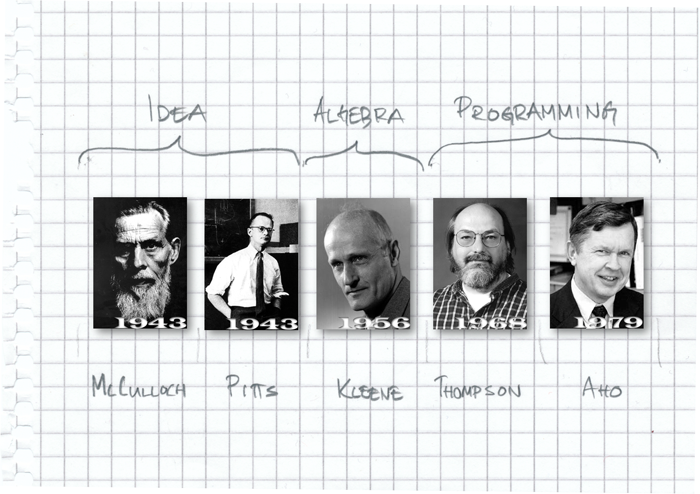
\includegraphics[width=1\textwidth]{images/history.png}
\end{frame}

\subsection{re module}
\begin{frame}
Delivering Quality since December 31, 1997 \\
\pause
Release of Python 1.5
\pause

\begin{itemize}
 \item Deprecated old module `regex`, based on Perl-style patterns.
\pause
 \item `regex` finally removed in Python 2.5 (September 19, 2006)
\end{itemize}
\end{frame}

\subsection{Do I need it?}
\begin{frame}
Answer for questions:
\pause
 \begin{itemize}
  \item "Does this string match the pattern?"
  \item "Is there a match for the pattern anywhere in this string?"
 \end{itemize}
 \pause
 \begin{itemize}
  \item Replace part of it
  \item Split into pieces
 \end{itemize}
\end{frame}

\subsection{Features}
\begin{frame}[fragile]
 re is handled as string  - there is no special syntax for expressing it (advantage and disadvantage) \\
 \pause
 re patterns are compiled into bytecode \\
 \pause
 re module is a C extension module (like \verb/socket/ or \verb/zlib/) \\
 \pause
 re language is relatively small and restricted
 \begin{itemize}
  \item not all possible string processing tasks can be done
  \item some of them can be done, but expression would be very complicated
 \end{itemize}
\end{frame}

\subsection{Regex Example}
\begin{frame}[fragile, allowframebreaks]
\begingroup
 \fontsize{6pt}{8pt}\selectfont
\begin{verbatim}
(?:(?:\r\n)?[ \t])*(?:(?:(?:[^()<>@,;:\\".\[\] \000-\031]+(?:(?:(?:\r\n)?[ \t]
)+|\Z|(?=[\["()<>@,;:\\".\[\]]))|"(?:[^\"\r\\]|\\.|(?:(?:\r\n)?[ \t]))*"(?:(?:
\r\n)?[ \t])*)(?:\.(?:(?:\r\n)?[ \t])*(?:[^()<>@,;:\\".\[\] \000-\031]+(?:(?:(
?:\r\n)?[ \t])+|\Z|(?=[\["()<>@,;:\\".\[\]]))|"(?:[^\"\r\\]|\\.|(?:(?:\r\n)?[
\t]))*"(?:(?:\r\n)?[ \t])*))*@(?:(?:\r\n)?[ \t])*(?:[^()<>@,;:\\".\[\] \000-\0
31]+(?:(?:(?:\r\n)?[ \t])+|\Z|(?=[\["()<>@,;:\\".\[\]]))|\[([^\[\]\r\\]|\\.)*\
](?:(?:\r\n)?[ \t])*)(?:\.(?:(?:\r\n)?[ \t])*(?:[^()<>@,;:\\".\[\] \000-\031]+
(?:(?:(?:\r\n)?[ \t])+|\Z|(?=[\["()<>@,;:\\".\[\]]))|\[([^\[\]\r\\]|\\.)*\](?:
(?:\r\n)?[ \t])*))*|(?:[^()<>@,;:\\".\[\] \000-\031]+(?:(?:(?:\r\n)?[ \t])+|\Z
|(?=[\["()<>@,;:\\".\[\]]))|"(?:[^\"\r\\]|\\.|(?:(?:\r\n)?[ \t]))*"(?:(?:\r\n)
?[ \t])*)*\<(?:(?:\r\n)?[ \t])*(?:@(?:[^()<>@,;:\\".\[\] \000-\031]+(?:(?:(?:\
r\n)?[ \t])+|\Z|(?=[\["()<>@,;:\\".\[\]]))|\[([^\[\]\r\\]|\\.)*\](?:(?:\r\n)?[
 \t])*)(?:\.(?:(?:\r\n)?[ \t])*(?:[^()<>@,;:\\".\[\] \000-\031]+(?:(?:(?:\r\n)
?[ \t])+|\Z|(?=[\["()<>@,;:\\".\[\]]))|\[([^\[\]\r\\]|\\.)*\](?:(?:\r\n)?[ \t]
)*))*(?:,@(?:(?:\r\n)?[ \t])*(?:[^()<>@,;:\\".\[\] \000-\031]+(?:(?:(?:\r\n)?[
 \t])+|\Z|(?=[\["()<>@,;:\\".\[\]]))|\[([^\[\]\r\\]|\\.)*\](?:(?:\r\n)?[ \t])*
)(?:\.(?:(?:\r\n)?[ \t])*(?:[^()<>@,;:\\".\[\] \000-\031]+(?:(?:(?:\r\n)?[ \t]
)+|\Z|(?=[\["()<>@,;:\\".\[\]]))|\[([^\[\]\r\\]|\\.)*\](?:(?:\r\n)?[ \t])*))*)
*:(?:(?:\r\n)?[ \t])*)?(?:[^()<>@,;:\\".\[\] \000-\031]+(?:(?:(?:\r\n)?[ \t])+
|\Z|(?=[\["()<>@,;:\\".\[\]]))|"(?:[^\"\r\\]|\\.|(?:(?:\r\n)?[ \t]))*"(?:(?:\r
\n)?[ \t])*)(?:\.(?:(?:\r\n)?[ \t])*(?:[^()<>@,;:\\".\[\] \000-\031]+(?:(?:(?:
\r\n)?[ \t])+|\Z|(?=[\["()<>@,;:\\".\[\]]))|"(?:[^\"\r\\]|\\.|(?:(?:\r\n)?[ \t
]))*"(?:(?:\r\n)?[ \t])*))*@(?:(?:\r\n)?[ \t])*(?:[^()<>@,;:\\".\[\] \000-\031
]+(?:(?:(?:\r\n)?[ \t])+|\Z|(?=[\["()<>@,;:\\".\[\]]))|\[([^\[\]\r\\]|\\.)*\](
?:(?:\r\n)?[ \t])*)(?:\.(?:(?:\r\n)?[ \t])*(?:[^()<>@,;:\\".\[\] \000-\031]+(?
:(?:(?:\r\n)?[ \t])+|\Z|(?=[\["()<>@,;:\\".\[\]]))|\[([^\[\]\r\\]|\\.)*\](?:(?
:\r\n)?[ \t])*))*\>(?:(?:\r\n)?[ \t])*)|(?:[^()<>@,;:\\".\[\] \000-\031]+(?:(?
:(?:\r\n)?[ \t])+|\Z|(?=[\["()<>@,;:\\".\[\]]))|"(?:[^\"\r\\]|\\.|(?:(?:\r\n)?
[ \t]))*"(?:(?:\r\n)?[ \t])*)*:(?:(?:\r\n)?[ \t])*(?:(?:(?:[^()<>@,;:\\".\[\]
\000-\031]+(?:(?:(?:\r\n)?[ \t])+|\Z|(?=[\["()<>@,;:\\".\[\]]))|"(?:[^\"\r\\]|
\\.|(?:(?:\r\n)?[ \t]))*"(?:(?:\r\n)?[ \t])*)(?:\.(?:(?:\r\n)?[ \t])*(?:[^()<>
@,;:\\".\[\] \000-\031]+(?:(?:(?:\r\n)?[ \t])+|\Z|(?=[\["()<>@,;:\\".\[\]]))|"
(?:[^\"\r\\]|\\.|(?:(?:\r\n)?[ \t]))*"(?:(?:\r\n)?[ \t])*))*@(?:(?:\r\n)?[ \t]
)*(?:[^()<>@,;:\\".\[\] \000-\031]+(?:(?:(?:\r\n)?[ \t])+|\Z|(?=[\["()<>@,;:\\
".\[\]]))|\[([^\[\]\r\\]|\\.)*\](?:(?:\r\n)?[ \t])*)(?:\.(?:(?:\r\n)?[ \t])*(?
:[^()<>@,;:\\".\[\] \000-\031]+(?:(?:(?:\r\n)?[ \t])+|\Z|(?=[\["()<>@,;:\\".\[
\]]))|\[([^\[\]\r\\]|\\.)*\](?:(?:\r\n)?[ \t])*))*|(?:[^()<>@,;:\\".\[\] \000-
\031]+(?:(?:(?:\r\n)?[ \t])+|\Z|(?=[\["()<>@,;:\\".\[\]]))|"(?:[^\"\r\\]|\\.|(
?:(?:\r\n)?[ \t]))*"(?:(?:\r\n)?[ \t])*)*\<(?:(?:\r\n)?[ \t])*(?:@(?:[^()<>@,;
:\\".\[\] \000-\031]+(?:(?:(?:\r\n)?[ \t])+|\Z|(?=[\["()<>@,;:\\".\[\]]))|\[([
^\[\]\r\\]|\\.)*\](?:(?:\r\n)?[ \t])*)(?:\.(?:(?:\r\n)?[ \t])*(?:[^()<>@,;:\\"
.\[\] \000-\031]+(?:(?:(?:\r\n)?[ \t])+|\Z|(?=[\["()<>@,;:\\".\[\]]))|\[([^\[\
]\r\\]|\\.)*\](?:(?:\r\n)?[ \t])*))*(?:,@(?:(?:\r\n)?[ \t])*(?:[^()<>@,;:\\".\
[\] \000-\031]+(?:(?:(?:\r\n)?[ \t])+|\Z|(?=[\["()<>@,;:\\".\[\]]))|\[([^\[\]\
r\\]|\\.)*\](?:(?:\r\n)?[ \t])*)(?:\.(?:(?:\r\n)?[ \t])*(?:[^()<>@,;:\\".\[\]
\000-\031]+(?:(?:(?:\r\n)?[ \t])+|\Z|(?=[\["()<>@,;:\\".\[\]]))|\[([^\[\]\r\\]
|\\.)*\](?:(?:\r\n)?[ \t])*))*)*:(?:(?:\r\n)?[ \t])*)?(?:[^()<>@,;:\\".\[\] \0
00-\031]+(?:(?:(?:\r\n)?[ \t])+|\Z|(?=[\["()<>@,;:\\".\[\]]))|"(?:[^\"\r\\]|\\
.|(?:(?:\r\n)?[ \t]))*"(?:(?:\r\n)?[ \t])*)(?:\.(?:(?:\r\n)?[ \t])*(?:[^()<>@,
;:\\".\[\] \000-\031]+(?:(?:(?:\r\n)?[ \t])+|\Z|(?=[\["()<>@,;:\\".\[\]]))|"(?
:[^\"\r\\]|\\.|(?:(?:\r\n)?[ \t]))*"(?:(?:\r\n)?[ \t])*))*@(?:(?:\r\n)?[ \t])*
(?:[^()<>@,;:\\".\[\] \000-\031]+(?:(?:(?:\r\n)?[ \t])+|\Z|(?=[\["()<>@,;:\\".
\[\]]))|\[([^\[\]\r\\]|\\.)*\](?:(?:\r\n)?[ \t])*)(?:\.(?:(?:\r\n)?[ \t])*(?:[
^()<>@,;:\\".\[\] \000-\031]+(?:(?:(?:\r\n)?[ \t])+|\Z|(?=[\["()<>@,;:\\".\[\]
]))|\[([^\[\]\r\\]|\\.)*\](?:(?:\r\n)?[ \t])*))*\>(?:(?:\r\n)?[ \t])*)(?:,\s*(
?:(?:[^()<>@,;:\\".\[\] \000-\031]+(?:(?:(?:\r\n)?[ \t])+|\Z|(?=[\["()<>@,;:\\
".\[\]]))|"(?:[^\"\r\\]|\\.|(?:(?:\r\n)?[ \t]))*"(?:(?:\r\n)?[ \t])*)(?:\.(?:(
?:\r\n)?[ \t])*(?:[^()<>@,;:\\".\[\] \000-\031]+(?:(?:(?:\r\n)?[ \t])+|\Z|(?=[
\["()<>@,;:\\".\[\]]))|"(?:[^\"\r\\]|\\.|(?:(?:\r\n)?[ \t]))*"(?:(?:\r\n)?[ \t
])*))*@(?:(?:\r\n)?[ \t])*(?:[^()<>@,;:\\".\[\] \000-\031]+(?:(?:(?:\r\n)?[ \t
])+|\Z|(?=[\["()<>@,;:\\".\[\]]))|\[([^\[\]\r\\]|\\.)*\](?:(?:\r\n)?[ \t])*)(?
:\.(?:(?:\r\n)?[ \t])*(?:[^()<>@,;:\\".\[\] \000-\031]+(?:(?:(?:\r\n)?[ \t])+|
\Z|(?=[\["()<>@,;:\\".\[\]]))|\[([^\[\]\r\\]|\\.)*\](?:(?:\r\n)?[ \t])*))*|(?:
[^()<>@,;:\\".\[\] \000-\031]+(?:(?:(?:\r\n)?[ \t])+|\Z|(?=[\["()<>@,;:\\".\[\
]]))|"(?:[^\"\r\\]|\\.|(?:(?:\r\n)?[ \t]))*"(?:(?:\r\n)?[ \t])*)*\<(?:(?:\r\n)
?[ \t])*(?:@(?:[^()<>@,;:\\".\[\] \000-\031]+(?:(?:(?:\r\n)?[ \t])+|\Z|(?=[\["
()<>@,;:\\".\[\]]))|\[([^\[\]\r\\]|\\.)*\](?:(?:\r\n)?[ \t])*)(?:\.(?:(?:\r\n)
?[ \t])*(?:[^()<>@,;:\\".\[\] \000-\031]+(?:(?:(?:\r\n)?[ \t])+|\Z|(?=[\["()<>
@,;:\\".\[\]]))|\[([^\[\]\r\\]|\\.)*\](?:(?:\r\n)?[ \t])*))*(?:,@(?:(?:\r\n)?[
 \t])*(?:[^()<>@,;:\\".\[\] \000-\031]+(?:(?:(?:\r\n)?[ \t])+|\Z|(?=[\["()<>@,
;:\\".\[\]]))|\[([^\[\]\r\\]|\\.)*\](?:(?:\r\n)?[ \t])*)(?:\.(?:(?:\r\n)?[ \t]
)*(?:[^()<>@,;:\\".\[\] \000-\031]+(?:(?:(?:\r\n)?[ \t])+|\Z|(?=[\["()<>@,;:\\
".\[\]]))|\[([^\[\]\r\\]|\\.)*\](?:(?:\r\n)?[ \t])*))*)*:(?:(?:\r\n)?[ \t])*)?
(?:[^()<>@,;:\\".\[\] \000-\031]+(?:(?:(?:\r\n)?[ \t])+|\Z|(?=[\["()<>@,;:\\".
\[\]]))|"(?:[^\"\r\\]|\\.|(?:(?:\r\n)?[ \t]))*"(?:(?:\r\n)?[ \t])*)(?:\.(?:(?:
\r\n)?[ \t])*(?:[^()<>@,;:\\".\[\] \000-\031]+(?:(?:(?:\r\n)?[ \t])+|\Z|(?=[\[
"()<>@,;:\\".\[\]]))|"(?:[^\"\r\\]|\\.|(?:(?:\r\n)?[ \t]))*"(?:(?:\r\n)?[ \t])
*))*@(?:(?:\r\n)?[ \t])*(?:[^()<>@,;:\\".\[\] \000-\031]+(?:(?:(?:\r\n)?[ \t])
+|\Z|(?=[\["()<>@,;:\\".\[\]]))|\[([^\[\]\r\\]|\\.)*\](?:(?:\r\n)?[ \t])*)(?:\
.(?:(?:\r\n)?[ \t])*(?:[^()<>@,;:\\".\[\] \000-\031]+(?:(?:(?:\r\n)?[ \t])+|\Z
|(?=[\["()<>@,;:\\".\[\]]))|\[([^\[\]\r\\]|\\.)*\](?:(?:\r\n)?[ \t])*))*\>(?:(
?:\r\n)?[ \t])*))*)?;\s*)
\end{verbatim}
 \endgroup
Perl regex to validate email addresses according to the RFC 822
\url{http://ex-parrot.com/~pdw/Mail-RFC822-Address}
\end{frame}

\subsection{The Dragon}
\begin{frame}[fragile]
\begin{lstlisting}
([0-9]+) (\w+ \w+)\n(?P<city>[\w ]+), ([A-Z]{2}) (?P<zip>\d{5})
\end{lstlisting}
\end{frame}

\section{Beginning}
\subsection{Compilation Process}
\begin{frame}[fragile]
\begin{lstlisting}
>>> import re
>>> re.findall('[a-zA-Z0-9]+', 'Search test 03')
['Search', 'test', '03']
\end{lstlisting}
\begin{lstlisting}
>>> import re
>>> regex = re.compile('[a-zA-Z0-9]+')
>>> regex
re.compile('[a-zA-Z0-9]+')
>>> re.findall(regex, 'Search test 02')
['Search', 'test', '02']
\end{lstlisting}
\begin{lstlisting}
>>> import re
>>> regex = re.compile('[a-zA-Z0-9]+')
>>> regex
re.compile('[a-zA-Z0-9]+')
>>> regex.findall('Search test 01')
['Search', 'test', '01']
\end{lstlisting}
\end{frame}

\subsection{Flags}
\begin{frame}[fragile]
\begin{itemize}
\item \verb/re.DEBUG/
\item \verb/re.ASCII, re.A/
\item \verb/re.IGNORECASE, re.I/
\item \verb/re.MULTILINE, re.M/
\item \verb/re.DOTALL, re.S/
\item \verb/re.VERBOSE, re.X/
\item \verb/re.LOCALE, re.L/ \textit{Do not use. Deprecated in Py3.5, will be removed in Py3.6}
\end{itemize}
\end{frame}

\subsection{Metacharacters}
\begin{frame}[fragile]
\begin{verbatim}
. ^ $ * + ? { } [ ] \ | ( )
\end{verbatim}
\end{frame}

\subsection{Repeating Things}
\subsubsection{*, +, ?}
\begin{frame}[fragile]
\verb/*/ - asterisk. Specifies that previous character can be matched zero or more times.
\begin{lstlisting}
>>> re.findall("ca*t", "ct, cat, caat")
['ct', 'cat', 'caat']
\end{lstlisting}
\pause
\verb/+/ - plus. Similar to \verb/*/, but requires at least one occurence of character.
\begin{lstlisting}
>>> re.findall("ca+t", "ct, cat, caat")
['cat', 'caat']
\end{lstlisting}
\pause
\verb/?/ - question mark. Matches either once or zero times
\begin{lstlisting}
>>> re.findall("ca?t", "ct, cat, caat")
['ct', 'cat']
\end{lstlisting}
\pause
\begin{lstlisting}
>>> re.findall("home-?brew", "homebrew, home-brew")
['homebrew', 'home-brew']
\end{lstlisting}
\end{frame}

\subsubsection{"{m,n}"}
\begin{frame}[fragile]
\verb/{m,n}/ - \verb/m/ and \verb/n/ are decimal numbers. There must be at least m repetitions, and at most n.
\begin{lstlisting}
>>> re.findall("a/{1,2}b", "ab, a/b, a//b, a///b")
['a/b', 'a//b']
\end{lstlisting}
\pause
\verb/m/ and \verb/n/ can be ommited. When m ommited, there is zero, when n ommited, upper bound infinity (more precisely, 2 billions)
\end{frame}

\begin{frame}[fragile]
\frametitle{Equivalents}
\begin{verbatim}
{0,} == "*"
{1,} == "+"
{,1} == {0,1} == "?"
\end{verbatim}
\end{frame}

\subsection{Greedy vs. Non-greedy}
\begin{frame}[fragile]
\verb/*/, \verb/+/, \verb/?/ and \verb/{m,n}/ are greedy. Will try to repeat it as many times as possible (re engine can match only 2 billion characters (2GB) -- C \verb/int/ limitation). \\
\pause
\verb/a[bcd]*b/ - matches \verb/a/, zero or more letters from \verb/bcd/, and ends with \verb/b/ \\
\begin{center}
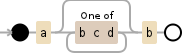
\includegraphics[width=0.5\textwidth]{images/greedy.png}
\end{center}
src: \url{https://www.debuggex.com/r/NT7_HIVhxI_h64zk}
\end{frame}

\begin{frame}[fragile]
\verb/re.match("a[bcd]*b", "abcbd")/
\begin{itemize}
\item matches \verb/a/
\pause
\item matches \verb/abcbd/ to the end of the string
\pause
\item fails, because current position is the end of the string, so cannot match \verb/b/
\pause
\item matches \verb/abcb/ - one less character
\pause
\item fails, because current position is \verb/d/, so cannot match \verb/b/
\pause
\item matches \verb/abc/, so \verb/[bcd]*/ matches only \verb/bc/
\pause
\item \verb/abcb/, tries last character \verb/b/, and it's on current position
\pause
\item success
\end{itemize}
\begin{lstlisting}
>>> re.findall('a[bcd]*b', 'abcbd')
['abcb']
\end{lstlisting}
\end{frame}

\begin{frame}[fragile]
\verb/*?, +?, ??, {m,n}?/ are non-greedy. Will try to match as few characters as possible.
\pause

\begin{lstlisting}
>>> import re
>>> text = "<html><head><title>Title</title></head></html>"
\end{lstlisting}
\pause
\begin{lstlisting}
>>> greedy_regex = re.compile("<.*>")
>>> greedy_regex.findall(text)
['<html><head><title>Title</title></head></html>']
\end{lstlisting}
\pause
\begin{lstlisting}
>>> non_greedy_regex = re.compile("<.*?>")
>>> non_greedy_regex.findall(text)
['<html>', '<head>', '<title>', '</title>', '</head>', '</html>']
>>>
\end{lstlisting}

\end{frame}

\subsection{Backslash - escape metacharacters}
\begin{frame}[fragile]
\verb/\/ - backslash (escape metacharacters) \\
For matching \verb/[/ or \verb/\/ you can use \verb/\[/ or \verb/\\/ \\
\begin{lstlisting}
>>> re.findall("\[\]", "Find brackets []")
['[]']
\end{lstlisting}
\pause
Some of special sequences beginning with \verb/\/ express predefined sets of characters: set of digits, letters, everything but whitespace
\end{frame}

\subsection{"Backslash Plague" problem}
\begin{frame}[fragile]
\begin{itemize}
\item re is handled as string
\pause
\item one of \verb/re/ metacharacters is \verb/\/
\pause
\item backslash for escaping in \verb/re/ conflicts with the same purpose in Python
\end{itemize}
\end{frame}

\begin{frame}[fragile]
\begin{tabular}{ | l | p{7cm} |}
\hline
Characters & Stage \\ \hline
\verb/\section/ & Text string to be matched \\
\verb/\\section/ & Escaped backslash for \verb/re.compile()/ \\
\verb/"\\\\section"/ & Escaped backslashes for a string literal \\
\hline
\end{tabular}
\pause
re string needs to be written as \verb/"\\\\"/ because regular expression must be \verb/\\/ and each must be escaped \verb/\\/ inside a regular Python string literal. \\
\pause
Solution - raw string
\begin{tabular}{ | l | p{7cm} |}
\hline
Regular string & Raw string \\ \hline
\verb/"ab*"/ & \verb/r"ab*"/ \\
\verb/"\\\\section"/ & \verb/r"\\section"/ \\
\verb/"\\w+\\s+"/ & \verb/r"\w+\s+"/ \\
\hline
\end{tabular}
\end{frame}

\section{Features}
\subsection{Performing Matches}
\subsubsection{match() vs. search()}
\begin{frame}[fragile]
\verb/match()/ vs. \verb/search()/
\begin{lstlisting}
>>> text = 'Your own personal Jesus Someone to hear your prayers Someone who cares Your own personal Jesus'
\end{lstlisting}
\begin{lstlisting}
>>> re.search("Your", text)
<_sre.SRE_Match object; span=(0, 4), match='Your'>
\end{lstlisting}
\begin{lstlisting}
>>> re.match("Your", text)
<_sre.SRE_Match object; span=(0, 4), match='Your'>
\end{lstlisting}
\begin{lstlisting}
>>> re.search("Jesus", text)
<_sre.SRE_Match object; span=(18, 23), match='Jesus'>
\end{lstlisting}
\begin{lstlisting}
>>> re.match("Jesus", text)
>>>
\end{lstlisting}
\end{frame}

\subsection{Grouping}
\subsubsection{Introduction}
\begin{frame}[fragile]
\begin{lstlisting}
>>> date = "10 December 2015"
>>> matched = re.match("(\d+) (\w+) (\d{4})", date)
>>> matched.groups()
('10', 'December', '2015')
>>> matched.group(1)
'10'
>>> matched.group(2)
'December'
>>> matched.group(3)
'2015'
>>>
\end{lstlisting}
\end{frame}

\subsubsection{Named groups}
\begin{frame}[fragile]
\begin{lstlisting}
>>> date = "10 December 2015"
>>> matched = re.match("(?P<day>\d+) (?P<month>\w+) (?P<year>\d{4})", date)
>>> matched.groups()
('10', 'December', '2015')
>>> matched.group('day')
'10'
>>> matched.group('month')
'December'
>>> matched.group('year')
'2015'
>>> matched.groupdict()
{'month': 'December', 'day': '10', 'year': '2015'}
>>>
\end{lstlisting}
\end{frame}

\subsection{Engines comparison}
\begin{frame}
\begin{center}
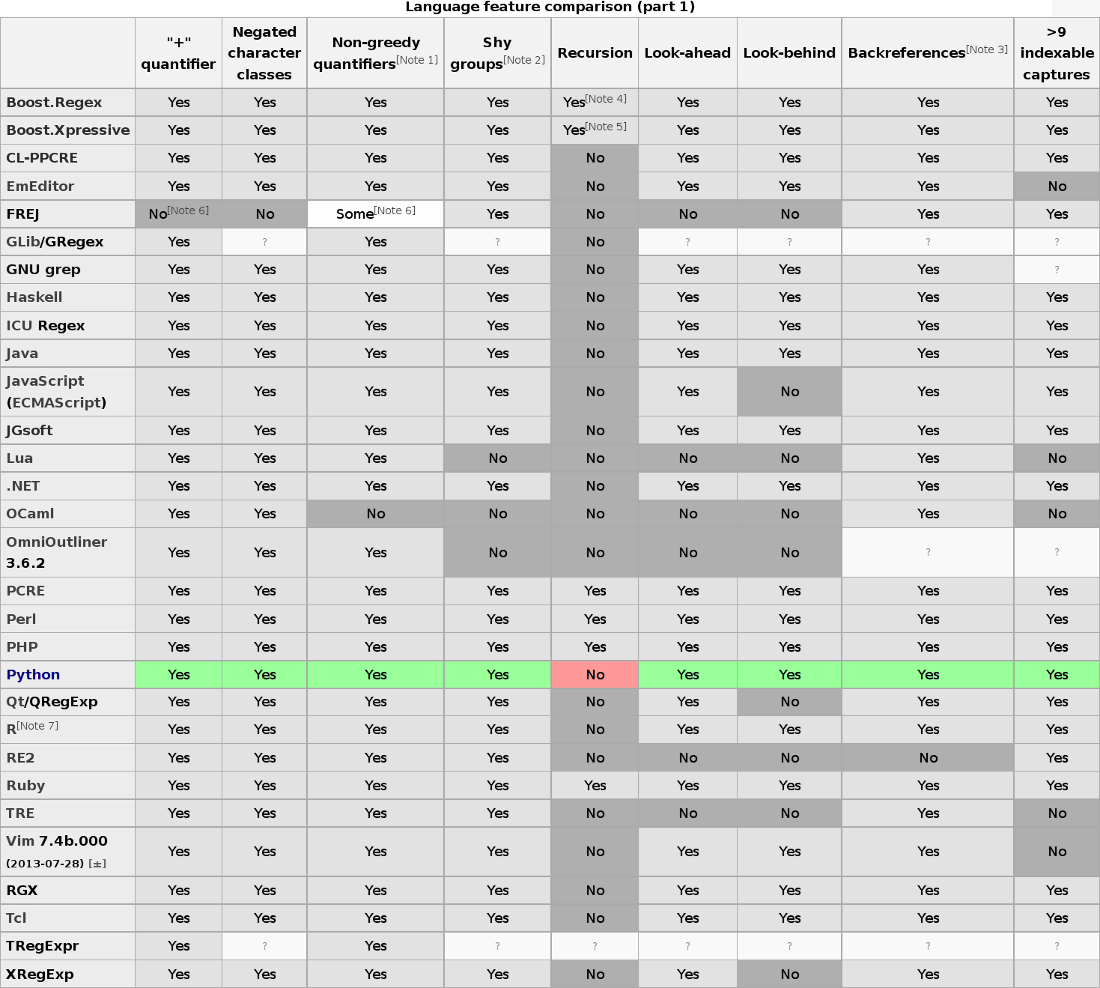
\includegraphics[width=1\textwidth]{images/re1.png}
\end{center}
\end{frame}

\begin{frame}
\begin{center}
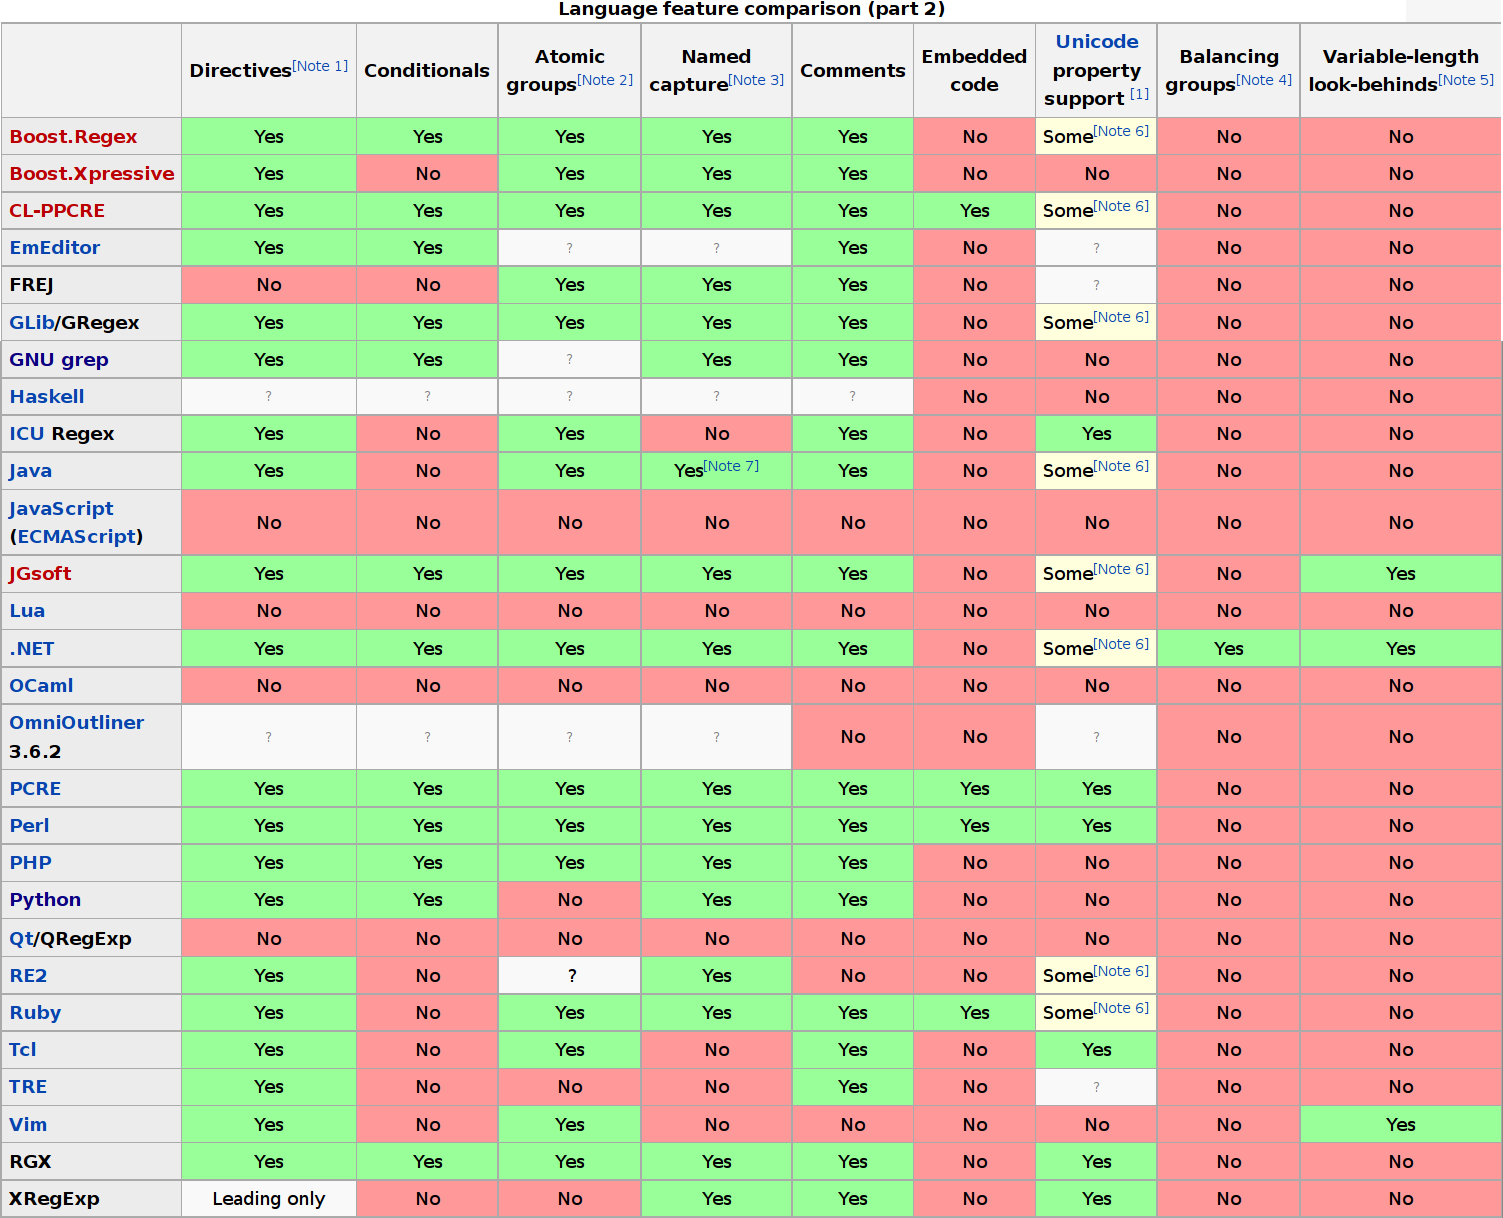
\includegraphics[width=1\textwidth]{images/re2.png}
\end{center}
\end{frame}

\subsection{Slaying the Dragon}
\begin{frame}[fragile]
\begin{lstlisting}
([0-9]+) (\w+\ \w+)\n(?P<city>[\w ]+), ([A-Z]{2}) (?P<zip>\d{5})
\end{lstlisting}
\end{frame}

\begin{frame}[fragile]
\begin{lstlisting}
def verify_regex(text):
    regex = """
    ([0-9]+)     # Match any recurring numbers
    \            # One whitespace
    (\w+ \w+)    # Match street
    \n           # New line
    (?P<city>[\w ]+) # Named group for City
    ,            # Comma :)
    \            # One whitespace
    ([A-Z]{2})   # Two capital letters, matching state
    \            # One whitespace
    (?P<zip>\d{5}) # Named group for matching ZIP code
    """
    re_compile = re.compile(regex, re.X)
    matched = re_compile.match(text)
    print(matched.groups())
\end{lstlisting}
\end{frame}

\begin{frame}[fragile]
\begin{lstlisting}
>>> address = """1 Fanatical Place
San Antonio, TX 78218"""
>>> verify_regex(address)
('1', 'Fanatical Place', 'San Antonio', 'TX', '78218')
>>>
\end{lstlisting}
\end{frame}

\subsection{Why am I talking about this?}
\begin{frame}[fragile]
\begin{lstlisting}
def parse_volume_type_from_filename(self, emcConfigFile):
    """Parse the volume type from the file (if it exists).

    :param emcConfigFile: the EMC configuration file
    :returns: volumeTypeName - the volume type name
    """
    volumeTypeName = None

    m = re.search('/etc/cinder/cinder_emc_config_(.+?).xml', emcConfigFile)
    if m:
        volumeTypeName = m.group(1)

    return volumeTypeName
"cinder/cinder/volume/drivers/emc/emc_vmax_utils.py"
\end{lstlisting}
\end{frame}

\section{Competition}
\subsection{PyPI}
\begin{frame}
\begin{center}
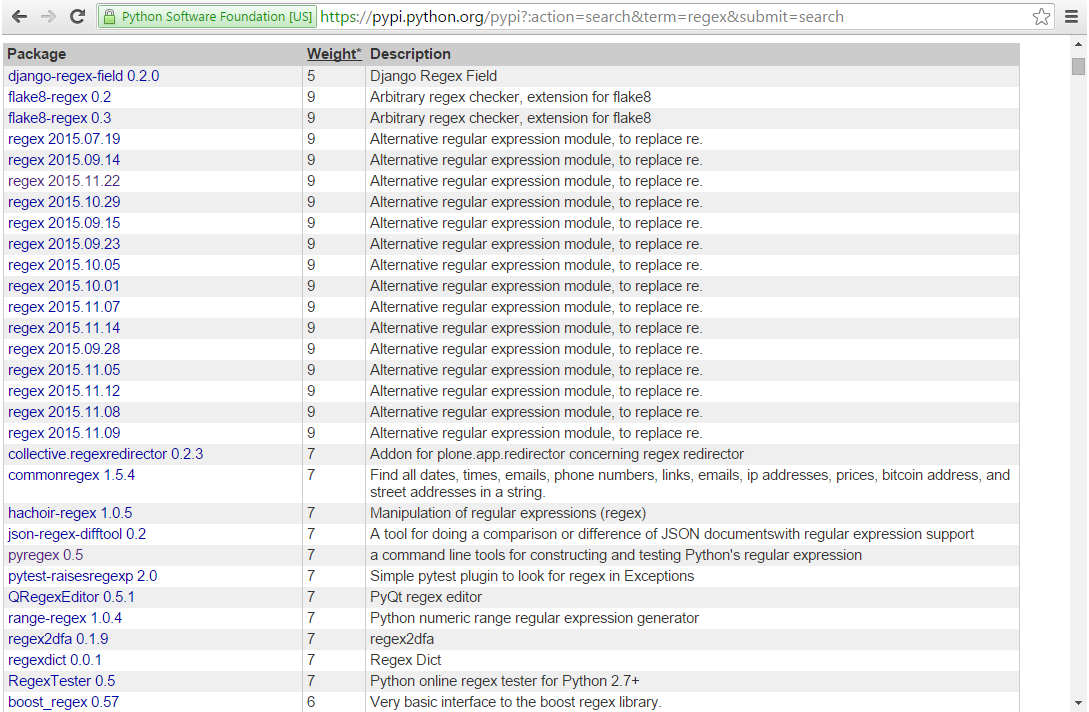
\includegraphics[width=1\textwidth]{images/regex_pypi.png}
\end{center}
\end{frame}

\subsection{re2}
\begin{frame}
Wrapper for Google RE2 engine
\\
Prerequisites for re2 in Python:
\begin{itemize}
\item RE2 library from Google
\item Python development headers
\item build environment with g++
\end{itemize}
\end{frame}

\subsection{re2 by Facebook}
\begin{frame}[fragile]
Released in April 2015. In development since 2010. \\
Features
\begin{itemize}
\item \verb/fullmatch/ works like \verb/match/ but anchors the match at both the start and the end
\item \verb/test_(search|match|fullmatch)/ methods that work like \verb/(search|match|fullmatch)/ but only returns \verb/True/ or \verb/False/
\end{itemize}
\end{frame}

\begin{frame}[fragile]
Missing Features
\begin{itemize}
\item no substitution methods
\item no flags
\item no \verb/split/, \verb/findall/, \verb/finditer/
\item no top-level functions like \verb/search/ or \verb/match/; just use compile
\item no compile cache
\item no \verb/lastindex/ or \verb/lastgroup/ on \verb/Match/ objects
\end{itemize}
\end{frame}

\subsection{re2 by Axiak}
\begin{frame}[fragile]
Initially fork of Facebook version, later rewritten from scratch. \\
Features
\begin{itemize}
\item Backward compatibility
\end{itemize}
\begin{lstlisting}
try:
    import re2 as re
except ImportError:
    import re
\end{lstlisting}
\verb/re2/ will automatically fall back to the original \verb/re/ module if there is a regex that it cannot handle: \verb/re2/ doesn't handle lookahead assertions \verb/(?=...)/.
\end{frame}

\begin{frame}
Missing Features/Flaws
\begin{itemize}
\item Unicode support: module supports UTF8, so automatically encodes and decodes any unicode string.
\end{itemize}
\end{frame}

\subsection{Why re2?}
\begin{frame}[fragile]
Total runs: 100
\begin{tabular}{ | l | l | l | l | }
\hline
Test & \verb/re/ time (s) & \verb/re2/ time (s) & \% time \\ \hline
Findall URI or Emails & 348.380 & 8.139 & 2.34\% \\
Replace wikilinks & 3.659 & 0.812 & 22.19\% \\
Remove wikilinks & 3.553 & 0.273 & 7.70\% \\
\hline
\end{tabular}
src: \url{https://github.com/axiak/pyre2/blob/master/tests/performance.py}
\end{frame}

\section{Wrap-up}
\subsection{Bibliography}
\begin{frame}[allowframebreaks]
\begingroup
\fontsize{6pt}{8pt}\selectfont
\begin{itemize}
\item Regular Expression HOWTO: \url{https://docs.python.org/2/howto/regex.html}
\item Python Docs: Library re: \url{https://docs.python.org/2/library/re.html}
\item Google for Education. Python Regular Expressions: \url{https://developers.google.com/edu/python/regular-expressions?hl=en}
\item Regex Debugger: \url{https://regex101.com/}
\item Debuggex: \url{https://www.debuggex.com/}
\item Core Python Applications programming: Regular expressions: \url{http://www.informit.com/articles/article.aspx?p=1707750&seqNum=2}
\item Brief history by Staffan Noteberg: \url{http://blog.staffannoteberg.com/}
\item Regular Expression Matching Can Be Simple And Fast \url{https://swtch.com/~rsc/regexp/regexp1.html}
\end{itemize}

\begin{itemize}
\item Google RE2: \url{https://github.com/google/re2}
\item Facebook re2: \url{https://github.com/facebook/pyre2}
\item Axiak re2: \url{https://github.com/axiak/pyre2}
\item re2 on PyPI: \url{https://pypi.python.org/pypi/re2}
\end{itemize}
\endgroup
\end{frame}

\subsection{Thank you}
\begin{frame}
\frametitle{Thank you}
Questions?
\end{frame}

\end{document}
